\documentclass{article}
\usepackage[utf8]{inputenc}

\documentclass[a4paper]{article}
\usepackage[12pt]{extsizes}
\usepackage{amsmath,amsthm,amssymb}
\usepackage[hidelinks]{hyperref} 
\usepackage[warn]{mathtext}
\usepackage[T1,T2A]{fontenc}
\usepackage[utf8]{inputenc}
\usepackage[english,russian]{babel}
\usepackage{tocloft}
\linespread{1.5}
\usepackage{indentfirst}
\usepackage{setspace}
%\полуторный интервал
\onehalfspacing

\newcommand{\RomanNumeralCaps}[1]
    {\MakeUppercase{\romannumeral #1}}

\usepackage{amssymb}

\usepackage{graphicx, float}
\graphicspath{{pictures/}}
\DeclareGraphicsExtensions{.pdf,.png,.jpg}
\usepackage[left=25mm,right=1cm,
    top=2cm,bottom=20mm,bindingoffset=0cm]{geometry}
\renewcommand{\cftsecleader}{\cftdotfill{\cftdotsep}}

\addto\captionsrussian{\renewcommand{\contentsname}{СОДЕРЖАНИЕ}}
\addto\captionsrussian{\renewcommand{\listfigurename}{СПИСОК ИЛЛЮСТРАЦИЙ}}

\usepackage{fancyhdr}
\usepackage[nottoc]{tocbibind}

\fancypagestyle{plain}{
\fancyhf{}
\renewcommand{\headrulewidth}{0pt}
\fancyhead[R]{\thepage}
}

\usepackage{blindtext}
\pagestyle{myheadings}
\usepackage{hyperref}

\begin{document}
\begin{titlepage}
  \begin{center}
    \large
    Санкт-Петербургский политехнический университет Петра Великого
    
    Институт прикладной математики и механики
    
    \textbf{Высшая школа прикладной математики и вычислительной физики}
    \vfill
    \textsc{\textbf{\Large{Отчёт по лабораторной работе №1}}}\\[5mm]
    \\ по дисциплине\\ <<Математическая статистика>>\\
\end{center}

\vfill

\begin{tabular}{l p{140} l}
Выполнила студентка \\группы 3630102/80401 && Мамаева Анастасия Сергеевна \\
\\
Проверил\\Доцент, к.ф.-м.н.& \hspace{0pt} &   Баженов Александр Николаевич \\\\
\end{tabular}

\hfill \break
\hfill \break
\begin{center} Санкт-Петербург \\2021 \end{center}
\thispagestyle{empty}
\end{titlepage}
\newpage
\newpage
\begin{center}
    \setcounter{page}{2}
    \tableofcontents
\end{center}
\newpage
\begin{center}
    \setcounter{page}{3}
    \listoffigures
\end{center}

\newpage

\section {Постановка задачи}
\noindent Для 5 распределений:
\begin{enumerate}
	\item $N(x, 0, 1)$ -- нормальное распределение
	\item $C(x, 0, 1)$ -- распределение Коши
	\item $L(x, 0, \frac{1}{\sqrt{2}})$ -- распределение Лапласа 
	\item $P(k, 10)$ -- распределение Пуассона
	\item $U(x, -\sqrt{3}, \sqrt{3})$ -- расномерное распределение
\end{enumerate}

\noindent Сгенерировать выборки размером 10, 50 и 1000 элементов.\newline Построить на одном рисунке гистограмму и график плотности распределения.

\section {Теория}

\subsection{Распределения}
	\begin{itemize}
		\item Нормальное распределение \begin{equation}
										  N(x, 0, 1) = \frac{1}{\sqrt{2\pi}}e^{\frac{-x^2}{2}} \label{norm} 
									   \end{equation}
		\item Распределение Коши \begin{equation}
									C(x, 0, 1) = \frac{1}{\pi}\frac{1}{x^2+1} \label{koshi}
								 \end{equation} 
		\item Распределение Лапласа \begin{equation}
									   L(x, 0, \frac{1}{\sqrt{2}}) = \frac{1}{\sqrt{2}}e^{-\sqrt{2}|x|} \label{laplace} 
									\end{equation}
		\item Распределение Пуассона \begin{equation}
										P(k, 10) = \frac{10^k}{k!}e^{-10}\label{puasson}
									 \end{equation}
		\item Равномерное распределение \begin{equation}
				U(x, -\sqrt{3}, \sqrt{3}) =
				\begin{cases}
					\frac{1}{2\sqrt{3}} &\text{$при |x|\leq \sqrt{3}$}\\
					0 &\text{$при |x|>\sqrt{3}$}
				\end{cases}
				\label{uni} 
			\end{equation}
	\end{itemize}

	\subsection{Гистограмма}
	\subsubsection{Определение}
	\noindent \textit{Гистограмма} в математической статистике — это функция, приближающая плотность вероятности некоторого распределения, построенная на основе выборки из него.
	
	\subsubsection{Графическое описание}
	\noindent Графически гистограмма строится следующим образом. Сначала множество значений, которое может принимать элемент выборки, разбивается на несколько интервалов. Чаще всего эти интервалы берут одинаковыми, но это не является строгим требованием. Эти интервалы откладываются на горизонтальной оси, затем над каждым рисуется прямоугольник. Если все интервалы были одинаковыми, то высота каждого прямоугольника пропорциональна числу элементов выборки, попадающих в соответствующий интервал. Если интервалы разные, то высота прямоугольника выбирается таким образом, чтобы его площадь была пропорциональна числу элементов выборки, которые попали в этот интервал.
	
	\subsubsection{Использование}
	\noindent Гистограммы применяются в основном для визуализации данных на начальном этапе статистической обработки. \newline Построение гистограмм используется для получения эмпирической оценки плотности распределения случайной величины. Для построения гистограммы наблюдаемый диапазон изменения случайной величины разбивается на несколько интервалов и подсчитывается доля от всех измерений, попавшая в каждый из интервалов. Величина каждой доли, отнесенная к величине интервала, принимается в качестве оценки значения плотности распределения на соответствующем интервале.

\section {Программная реализация} 	
\noindent Лабораторная работа выполнена на языке Python вресии 3.7 в среде разработки JupyterLab. Использовались дополнительные библиотеки:\\ \newline
1. scipy\newline
2. numpy\newline
3. matplotlib\newline
4. math\newline \\
В приложении находится ссылка на GitHub репозиторий с исходныи кодом.

\section {Результаты} 

\subsection{Гистограммы и графики плотности распределения}
	\begin{figure}[H]
		\centering
		\begin{tabular}{ccc}
			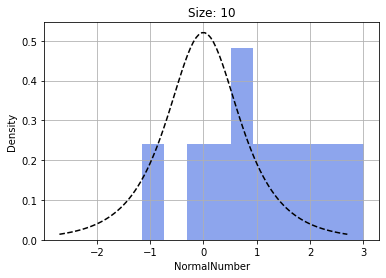
\includegraphics[width=55mm, height =0.25\textheight]{normalnumber10.png}
			&
			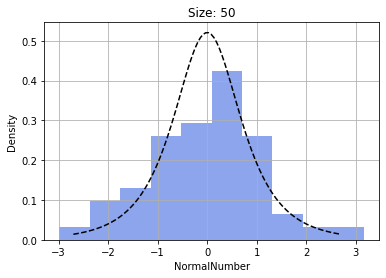
\includegraphics[width=55mm, height =0.25\textheight]{normalnumber50.png}
			&
			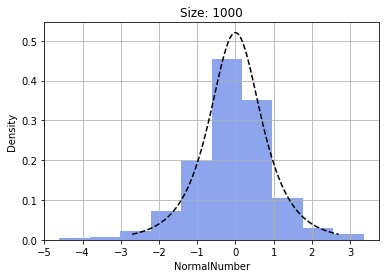
\includegraphics[width=55mm, height =0.25\textheight]{normalnumber1000.png}
		\end{tabular}
		\caption{Нормальное распределение \eqref{norm}} 
		\label{fig:normal}
	\end{figure}

	\begin{figure}[H]
		\centering
		\begin{tabular}{ccc}
			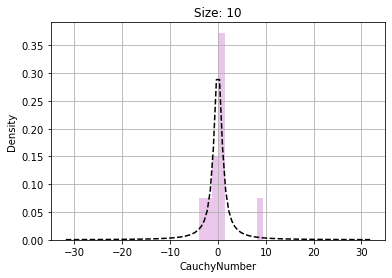
\includegraphics[width=55mm, height =0.25\textheight]{cauchynumber10.png}
			&
			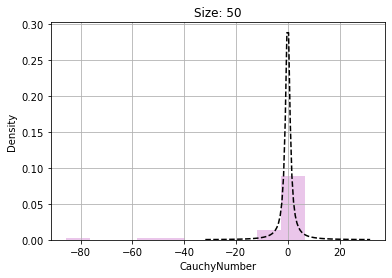
\includegraphics[width=55mm, height =0.25\textheight]{cauchynumber50.png}
			&
			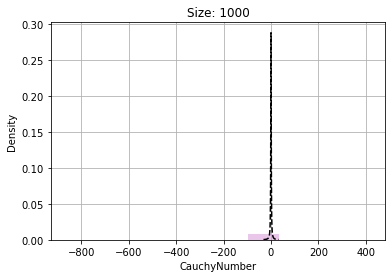
\includegraphics[width=55mm, height =0.25\textheight]{cauchynumber1000.png}
		\end{tabular}
		\caption{Распределение Коши \eqref{koshi}}
		\label{fig:cauchy}
	\end{figure}
	

	\begin{figure}[H]
		\centering
		\begin{tabular}{ccc}
			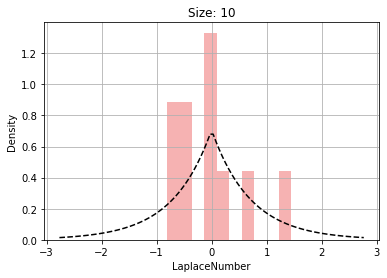
\includegraphics[width=55mm, height =0.25\textheight]{laplacenumber10.png}
			&
			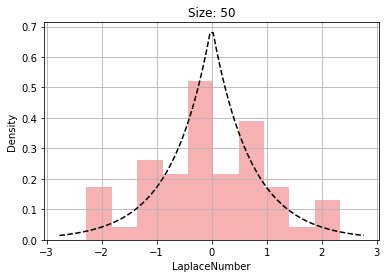
\includegraphics[width=55mm, height =0.25\textheight]{laplacenumber50.png}
			&
			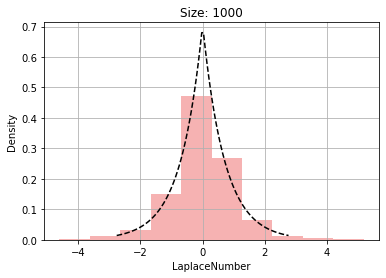
\includegraphics[width=55mm, height =0.25\textheight]{laplacenumber1000.png}
		\end{tabular}
		\caption{Распределение Лапласа \eqref{laplace}}
		\label{fig:laplace}
	\end{figure}


	\begin{figure}[H]
		\centering
		\begin{tabular}{ccc}
			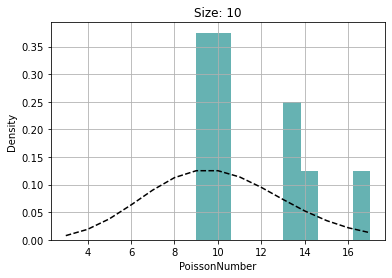
\includegraphics[width=55mm, height =0.25\textheight]{poissonnumber10.png}
			&
			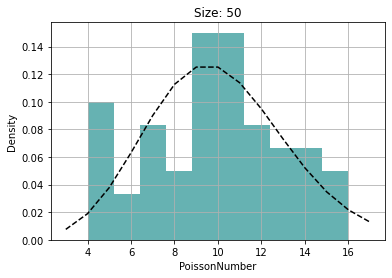
\includegraphics[width=55mm, height =0.25\textheight]{poissonnumber50.png}
			&
			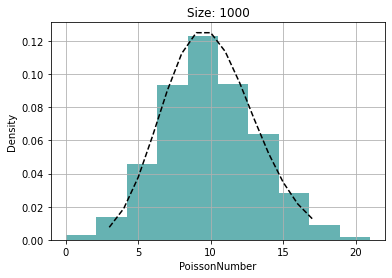
\includegraphics[width=55mm, height =0.25\textheight]{poissonnumber1000.png}
		\end{tabular}
		\caption{Распределение Пуассона \eqref{puasson}}
		\label{fig:poisson}
	\end{figure}


	\begin{figure}[H]
		\centering
		\begin{tabular}{ccc}
			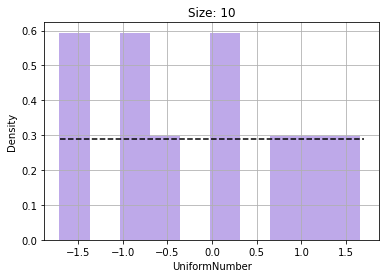
\includegraphics[width=55mm, height =0.25\textheight]{uniformnumber10.png}
			&
			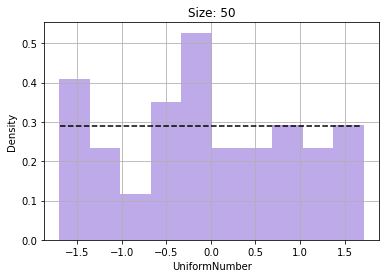
\includegraphics[width=55mm, height =0.25\textheight]{uniformnumber50.png}
			&
			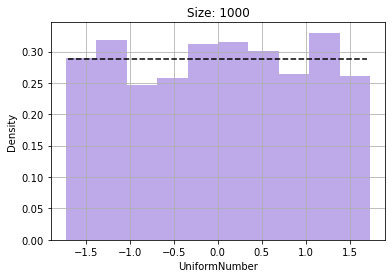
\includegraphics[width=55mm, height =0.25\textheight]{uniformnumber1000.png}
		\end{tabular}
		\caption{Равномерное распределение \eqref{uni}}
		\label{fig:uniform}
	\end{figure}

\section{Обсуждение}

\noindent По результатам проделанной работы можем сделать вывод о том, что чем больше выборка для каждого из распределений, тем ближе ее гистограмма к графику плотности вероятности того закона, по которому распределены величины сгенерированной выборки. Чем меньше выборка, тем менее она показательна - тем хуже по ней определяется характер распределения величины.\\\

\noindent Визуально очень трудно отличить гистограммы друг от друга, тем более при маленьких выборках. При выборке из 10 элементов вид гистрограммы много сильно отличается от плотности распределения. Чем больше выборка, тем точнее становится гистограмма. На выборке из 1000 элементов можем отличить  и распознать с большей вероятностью равномерное распределение (все прямоугольники примерно на одном уровне), а также распределение Пуассона (оно визуально шире чем распределение Лапласа и нормальное). Однако отличить между собой распределение Лапласа и нормальное тяжело. Так как визульно гистограммы получились похожи друг на друга и без подписей отличить их почти не представляется возможным.\\\
 
\noindent Также можно заметить, что максимумы гистограмм и плотностей распределения почти нигде не совпали. Из полученных графиков можно увидеть, что только при распределении Пуассона на выборке из 1000 элементов, максимум графика плотности вероятности совпал с максимумом гистограммы. Также наблюдаются всплески гистограмм, что наиболее хорошо прослеживается на распределении Коши. 

\section{Приложение}

\noindent Код программы GitHub URL:\\
\newline https://github.com/Brightest-Sunshine/Math-Statistic-2021/blob/main/Lab1/Lab1.ipynb

\end{document}
